\clearpage
\newpage
\chapter{Results}
\section{Limits}
\label{sec:bsstats}
We set limits on the production cross-section of 
the $\bs$ quark. We compare the number 
of observed events to the number of events expected given the new physics model. We use the following formula:
\begin{eqnarray}
N_{\textrm{expected}} = \sigma_{\bs} \times B_{\bs \rightarrow tW;W \to hadrons} \times \varepsilon \times \emph{L}
\end{eqnarray}
where $\sigma_{\bs}$ is the $\bs$ cross-section, $B_{\bs \rightarrow tW;W \to hadrons}$ is the branching ratio 
$\bs \to tW$ with both W boson decays constrained to the hadronic branching fraction, $\varepsilon$ is the efficiency and $\emph{L}$ is the integrated luminosity of our dataset. 

We perform a shape analysis using the $\mathrm{M_{tW}}$ distribution.  This analysis uses a binned likelihood fit to compare the distribution from the $\bs$ quark signal 
hypothesis with the SM distribution produced by our background estimation procedure.  

\label{sec:bsTheta}
We use a Bayesian method to extract 95\% CL upper limits 
on the production of a left- and right-handed $\bs$ particle.  

The statistical procedure for setting limits is described in Section~\ref{sec:stats}. 

The uncertainty in the jet energy scale, $Q^2$ scale, trigger, QCD background uncertainties, and jet energy resolution are taken 
as shape based uncertainties, and the other sources of uncertainty are taken as overall normalizations.  

The limits from Theta are shown in Figure \ref{figs:bsthetalimit}.  
The expected(observed) exclusion region for the right-handed $\bs$ quark hypothesis is between 0.88 TeV and 1.55 TeV (0.82 TeV and 1.43 TeV).  
The expected(observed) exclusion region for the left-handed $\bs$ quark hypothesis is between 0.89 TeV and 1.48 TeV (0.88 TeV and 1.40 TeV).  
The expected(observed) exclusion region for the vectorlike $\bs$ quark hypothesis is between 0.82 TeV and 1.70 TeV (0.8 TeV and 1.53 TeV).  Cross-section upper limits for 
right-handed, left-handed, and vectorlike $\bs$ are summarized in Tables \ref{table:bsupperxsecR},\ref{table:bsupperxsecL}, and \ref{table:bsupperxsecLR} respectively. 

Table \ref{table:bsnuisance} gives the values for nuisance parameters after limit setting for each $\bs$ mass hypothesis.

\begin{sidewaystable}
\begin{center}
\bf{Rate Effects of Systematic Uncertainties}\\
\scalebox{0.65}{
\begin{tabular}{c||c|c|c|c|c|c|c|c|c}
\hline\hline
\bf{Sample} & \bf{JER}  & \bf{JES} & \bf{$Q^2$} & \bf{QCD total} & \bf{Lumi} & \bf{top-tagging SF} & \bf{W-tagging SF} & \bf{Trigger}  & \bf{$\ttbar$ Norm} \\
\hline\hline
$M_{\bs}=1000$ & -0.81,+0.51 & +17.91,-21.34 & --- & --- & +2.63,-2.57 & +12.50,-11.11 & +7.60,-7.06 & +0.14,-0.14 & ---\\ 
$M_{\bs}=1100$ & -0.51,+0.60 & +9.07,-12.13 & --- & --- & +2.63,-2.57 & +12.50,-11.11 & +7.60,-7.06 & +0.07,-0.07 & ---\\ 
$M_{\bs}=1200$ & -0.41,+0.60 & +6.12,-9.76 & --- & --- & +2.63,-2.57 & +12.50,-11.11 & +7.60,-7.06 & +0.04,-0.04 & ---\\ 
$M_{\bs}=1300$ & -0.42,+0.41 & +4.98,-8.06 & --- & --- & +2.63,-2.57 & +12.50,-11.11 & +7.60,-7.06 & +0.03,-0.03 & ---\\ 
$M_{\bs}=1400$ & -0.53,+0.40 & +4.20,-7.65 & --- & --- & +2.63,-2.57 & +12.50,-11.11 & +7.60,-7.06 & +0.02,-0.02 & ---\\ 
$M_{\bs}=1500$ & -0.46,+0.42 & +4.50,-7.76 & --- & --- & +2.63,-2.57 & +12.50,-11.11 & +7.60,-7.06 & +0.02,-0.02 & ---\\ 
$M_{\bs}=1600$ & -0.48,+0.37 & +3.79,-7.33 & --- & --- & +2.63,-2.57 & +12.50,-11.11 & +7.60,-7.06 & +0.01,-0.01 & ---\\ 
$M_{\bs}=1700$ & -0.34,+0.35 & +3.91,-6.43 & --- & --- & +2.63,-2.57 & +12.50,-11.11 & +7.60,-7.06 & +0.01,-0.01 & ---\\ 
$M_{\bs}=1800$ & -0.48,+0.39 & +3.71,-7.64 & --- & --- & +2.63,-2.57 & +12.50,-11.11 & +7.60,-7.06 & +0.01,-0.01 & ---\\ 
$M_{\bs}=1900$ & -0.46,+0.44 & +3.31,-7.12 & --- & --- & +2.63,-2.57 & +12.50,-11.11 & +7.60,-7.06 & +0.01,-0.01 & ---\\ 
$M_{\bs}=2000$ & -0.46,+0.41 & +3.14,-7.29 & --- & --- & +2.63,-2.57 & +12.50,-11.11 & +7.60,-7.06 & +0.01,-0.01 & ---\\ 
$M_{\bs}=800$ & -0.00,+0.56 & +29.42,-25.25 & --- & --- & +2.63,-2.57 & +12.50,-11.11 & +7.60,-7.06 & +0.19,-0.19 & ---\\ 
$M_{\bs}=900$ & -0.18,+0.42 & +46.46,-35.69 & --- & --- & +2.63,-2.57 & +12.50,-11.11 & +7.60,-7.06 & +0.28,-0.28 & ---\\ 
qcd & --- & --- & --- & +28.14,-27.56 & --- & --- & --- & --- & ---\\ 
sts & +nan,+nan & +nan,+nan & --- & --- & +2.63,-2.57 & +12.50,-11.11 & +7.60,-7.06 & +nan,+nan & ---\\ 
stt & -0.11,+17.70 & +47.87,-16.85 & --- & --- & +2.63,-2.57 & +12.50,-11.11 & +7.60,-7.06 & +0.13,-0.13 & ---\\ 
sttW & +0.01,-0.00 & +17.42,-13.16 & --- & --- & +2.63,-2.57 & +12.50,-11.11 & +7.60,-7.06 & +0.09,-0.09 & ---\\ 
ttbar & -0.22,+1.05 & +13.20,-14.75 & +16.24,-23.58 & --- & --- & --- & +7.60,-7.06 & +0.10,-0.10 & +22.00,-18.03\\ 
\hline
\end{tabular}
}
\end{center}
\caption{Rate effects of the systematic uncertainties as extracted from Theta.  The numbers listed under sample specify $\bs$ signal MC mass.}
\label{table:bsnuisance}
\end{sidewaystable}



The cross section upper limits can be generalized due to the fact that the $\bs$ cross-section is dependent on the unknown constants $\kappa$ and $g$ as can be seen in equations \ref{eqn:Lag1} and \ref{eqn:Lag1}.
The limits can be extrapolated to the $g$,$\kappa$ plane as can be seen in figures \ref{figs:bsthetalimit2dobs} and \ref{figs:bsthetalimit2dobs} for observed and expected limits respectively.




\begin{table}
\begin{center}
\bf{$\bs_R$ Cross-Section Upper Limits}\\
\begin{tabular}{c||c|c|c|c}
\hline
\hline
\bf{$\mathrm{M_{\bs}}$} & \bf{observed}  & \bf{expected} & \bf{expected 1$\sigma$}  & \bf{expected 2$\sigma$} \\
\hline
\hline
800 & 3.298 & 6.325 & 3.584,11.675 & 1.999,22.481\\ 
900 & 0.283 & 0.549 & 0.323,0.953 & 0.202,1.961\\ 
1000 & 0.087 & 0.172 & 0.113,0.243 & 0.083,0.355\\ 
1100 & 0.122 & 0.112 & 0.077,0.162 & 0.056,0.223\\ 
1200 & 0.081 & 0.076 & 0.053,0.110 & 0.039,0.155\\ 
1300 & 0.051 & 0.052 & 0.036,0.077 & 0.026,0.107\\ 
1400 & 0.059 & 0.041 & 0.029,0.059 & 0.022,0.087\\ 
1500 & 0.062 & 0.034 & 0.024,0.049 & 0.017,0.071\\ 
1600 & 0.056 & 0.029 & 0.020,0.043 & 0.015,0.060\\ 
1700 & 0.035 & 0.025 & 0.018,0.038 & 0.013,0.053\\ 
1800 & 0.023 & 0.023 & 0.016,0.033 & 0.011,0.046\\ 
1900 & 0.021 & 0.022 & 0.015,0.031 & 0.011,0.044\\ 
2000 & 0.023 & 0.021 & 0.015,0.031 & 0.011,0.045\\ 
\hline
\end{tabular}
\end{center}
\caption{$\bs_R$ cross-section upper limits for given $\bs_R$ mass values.  Cross-section is in units of pb.}
\label{table:bsupperxsecR}
\end{table}

\begin{table}
\begin{center}
\bf{$\bs_L$ Cross-Section Upper Limits}\\
\begin{tabular}{c||c|c|c|c}
\hline\hline
\bf{$\mathrm{M_{\bs}}$} & \bf{observed}  & \bf{expected} & \bf{expected 1$\sigma$}  & \bf{expected 2$\sigma$} \\
\hline
\hline
800 & 7.681 & 8.588 & 5.106,15.127 & 2.798,27.319\\ 
900 & 0.355 & 0.674 & 0.395,1.211 & 0.237,2.369\\ 
1000 & 0.106 & 0.204 & 0.137,0.297 & 0.099,0.424\\ 
1100 & 0.148 & 0.140 & 0.096,0.200 & 0.069,0.273\\ 
1200 & 0.107 & 0.100 & 0.069,0.143 & 0.050,0.203\\ 
1300 & 0.068 & 0.067 & 0.047,0.102 & 0.035,0.140\\ 
1400 & 0.072 & 0.051 & 0.036,0.075 & 0.027,0.108\\ 
1500 & 0.081 & 0.045 & 0.031,0.066 & 0.023,0.092\\ 
1600 & 0.074 & 0.038 & 0.027,0.057 & 0.020,0.079\\ 
1700 & 0.049 & 0.034 & 0.023,0.050 & 0.017,0.070\\ 
1800 & 0.031 & 0.030 & 0.021,0.044 & 0.015,0.061\\ 
1900 & 0.028 & 0.029 & 0.021,0.041 & 0.015,0.058\\ 
2000 & 0.032 & 0.029 & 0.021,0.043 & 0.015,0.060\\ 
\hline
\end{tabular}
\end{center}
\caption{$\bs_L$ cross-section upper limits for given $\bs_L$ mass values.  Cross-section is in units of pb.}
\label{table:bsupperxsecL}
\end{table}


\begin{table}
\begin{center}
\bf{$\bs_{LR}$ Cross-Section Upper Limits}\\
\begin{tabular}{c||c|c|c|c}
\hline\hline
\bf{$\mathrm{M_{\bs}}$} & \bf{observed}  & \bf{expected} & \bf{expected 1$\sigma$}  & \bf{expected 2$\sigma$} \\
\hline
\hline
800 & 3.917 & 6.568 & 4.072,11.122 & 2.342,18.857\\ 
900 & 0.317 & 0.603 & 0.361,1.048 & 0.219,2.099\\ 
1000 & 0.095 & 0.187 & 0.124,0.269 & 0.087,0.386\\ 
1100 & 0.131 & 0.124 & 0.085,0.182 & 0.063,0.244\\ 
1200 & 0.094 & 0.086 & 0.060,0.124 & 0.044,0.177\\ 
1300 & 0.059 & 0.059 & 0.041,0.088 & 0.031,0.121\\ 
1400 & 0.065 & 0.046 & 0.033,0.066 & 0.024,0.097\\ 
1500 & 0.070 & 0.039 & 0.027,0.056 & 0.019,0.082\\ 
1600 & 0.065 & 0.033 & 0.023,0.049 & 0.017,0.069\\ 
1700 & 0.042 & 0.029 & 0.020,0.043 & 0.014,0.059\\ 
1800 & 0.026 & 0.026 & 0.018,0.038 & 0.013,0.053\\ 
1900 & 0.025 & 0.025 & 0.017,0.035 & 0.013,0.051\\ 
2000 & 0.026 & 0.025 & 0.017,0.036 & 0.013,0.050\\ 
\hline
\end{tabular}
\end{center}
\caption{$\bs_{LR}$ cross-section upper limits for given $\bs_{LR}$ mass values.  Cross-section is in units of pb.}
\label{table:bsupperxsecLR}
\end{table}


\begin{figure}[htcb]
\centering
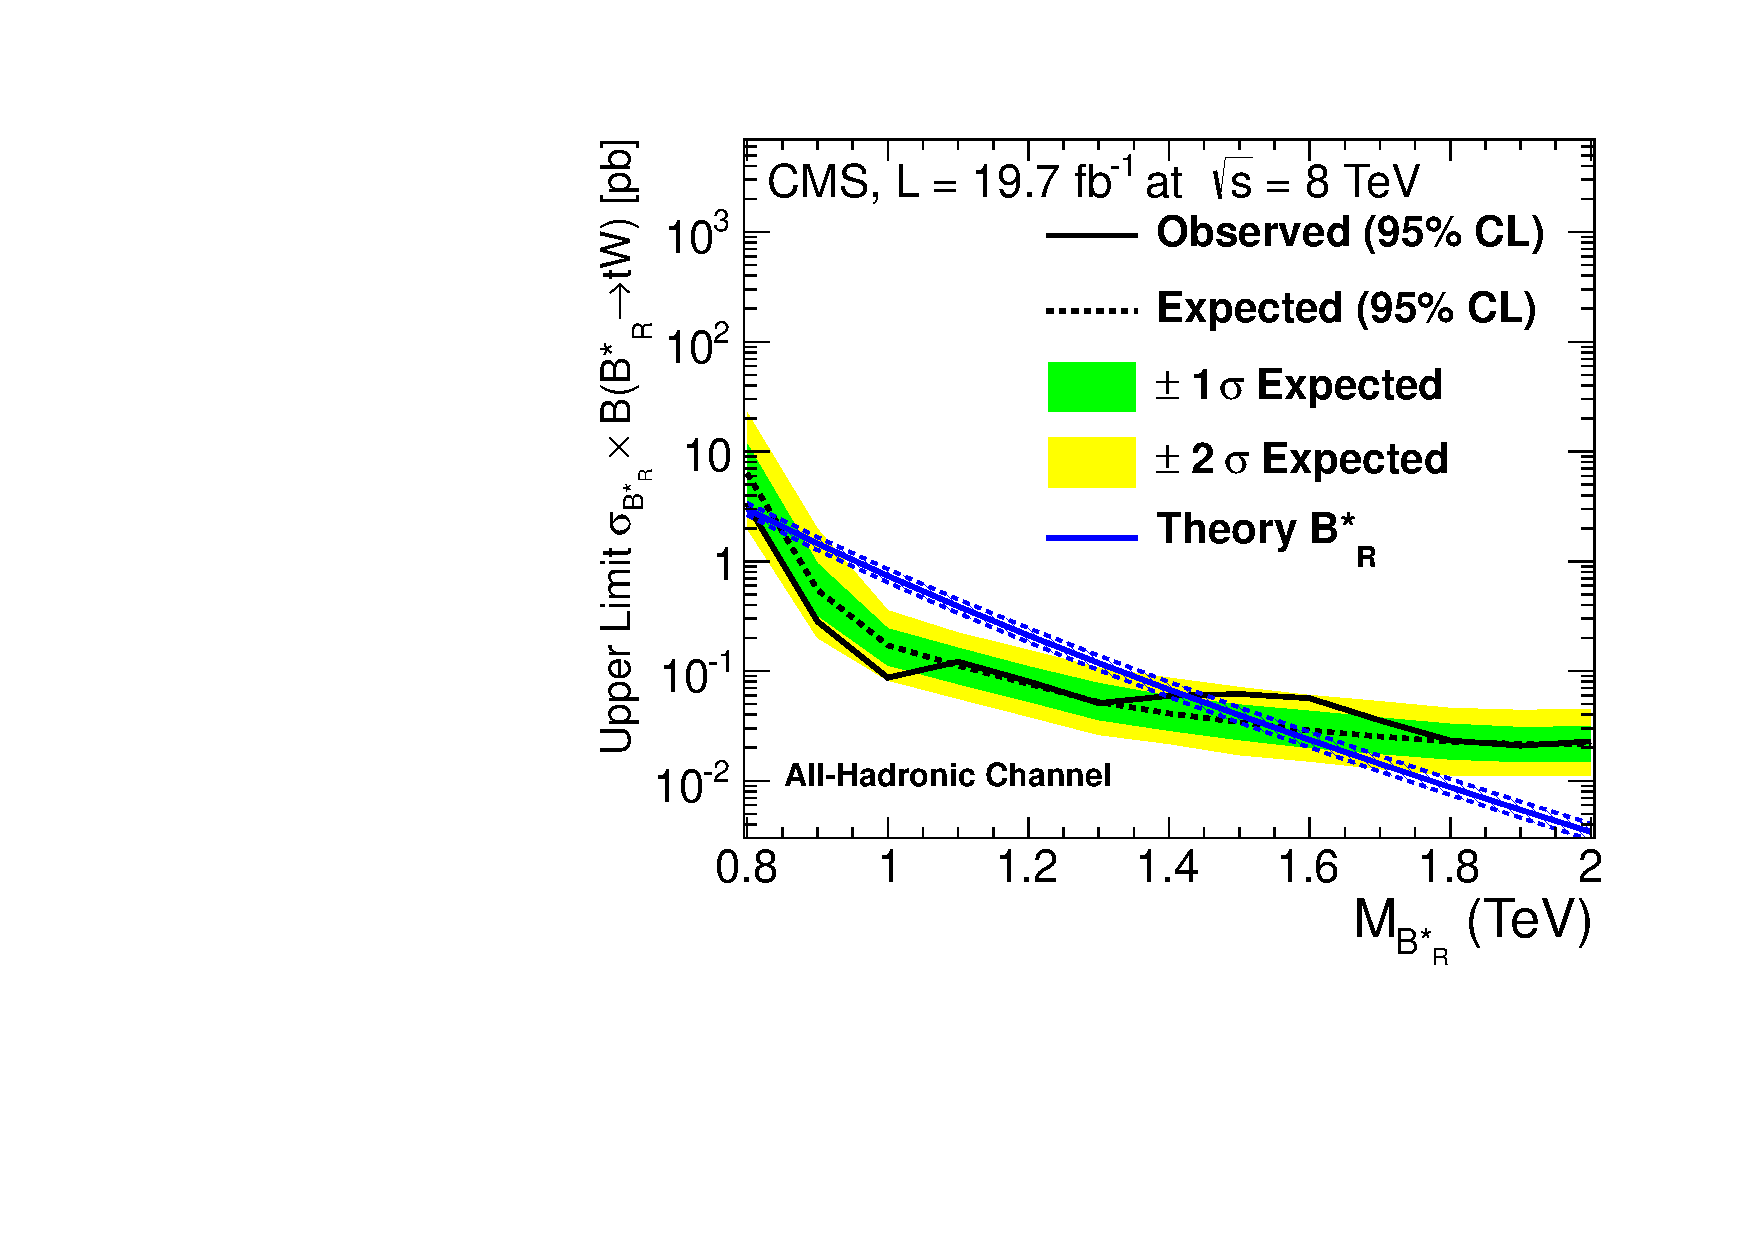
\includegraphics[width=0.45\textwidth]{AN-14-049/figs/limits_theta_had_right_log.pdf}\\
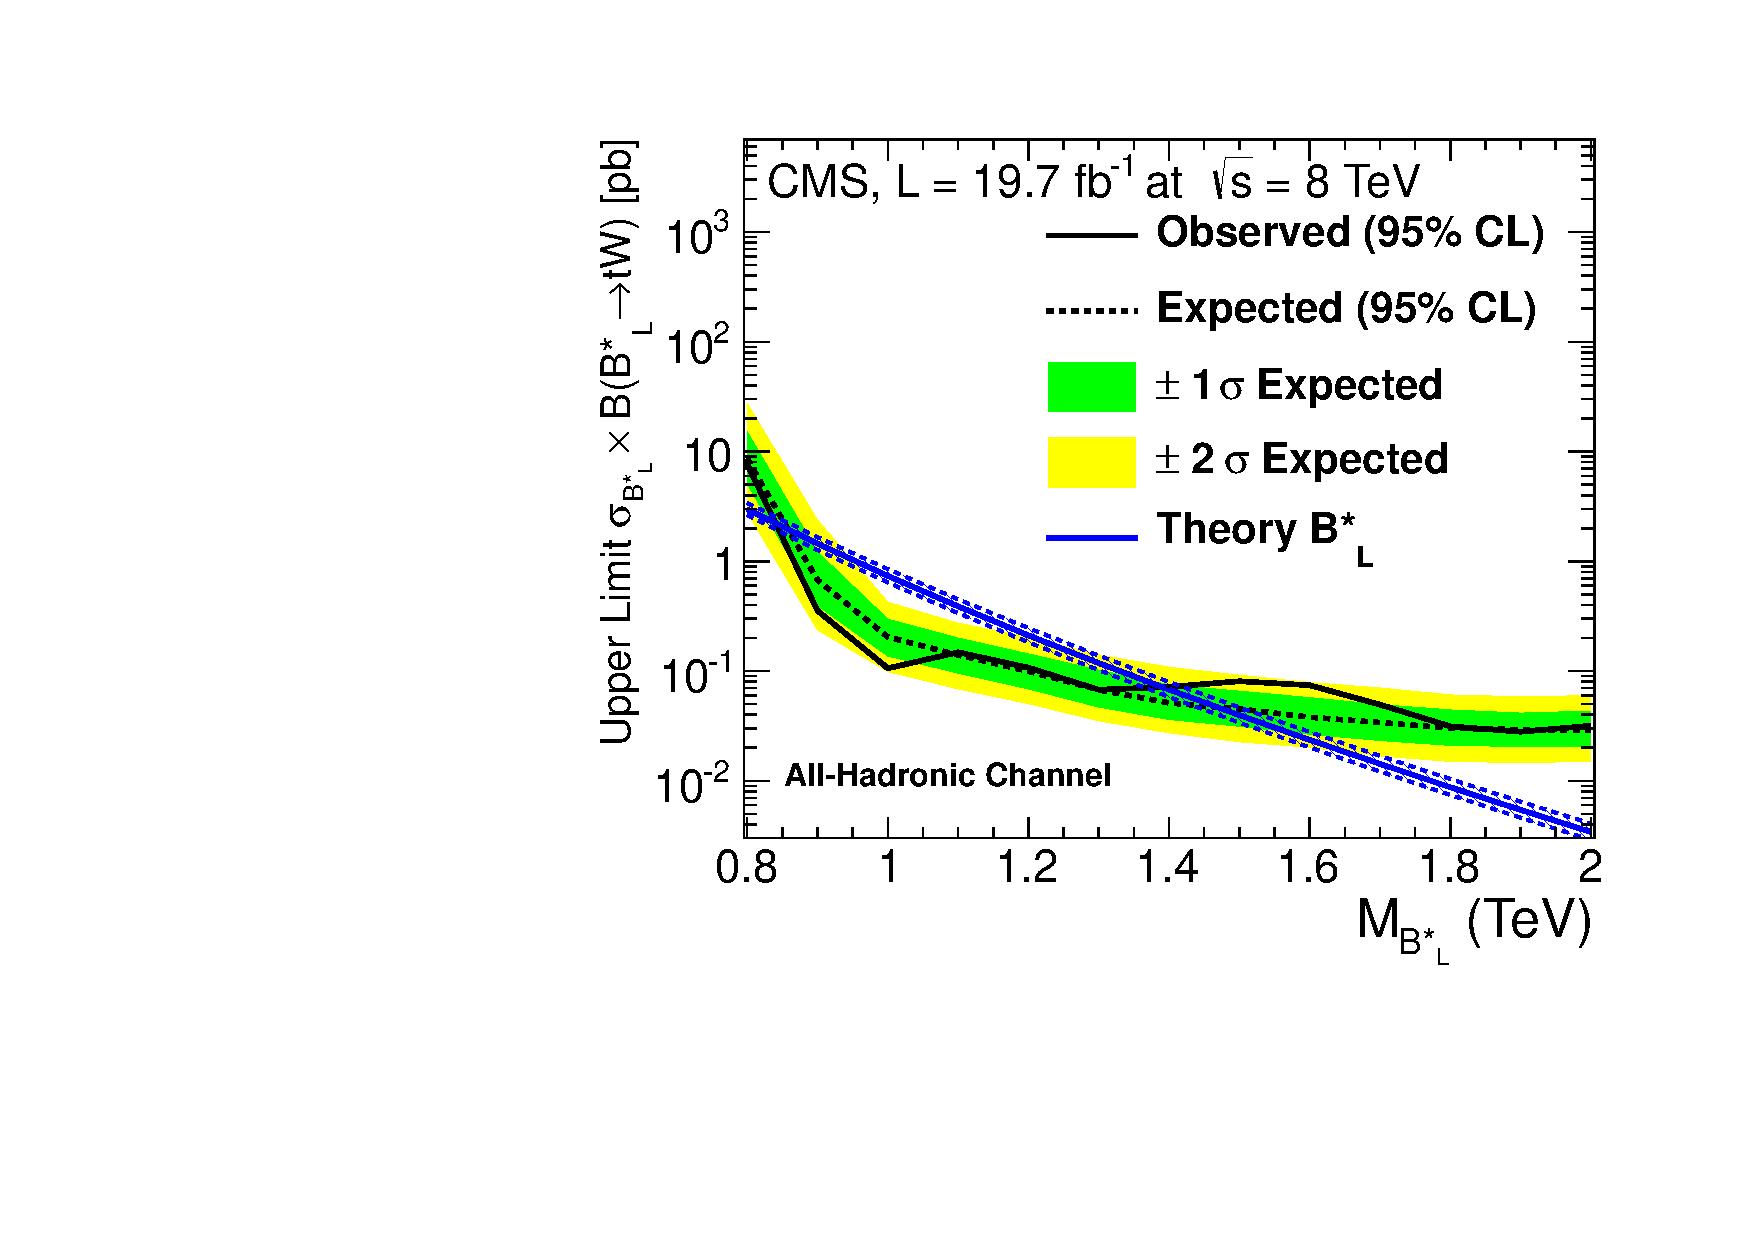
\includegraphics[width=0.45\textwidth]{AN-14-049/figs/limits_theta_had_left_log.pdf}\\
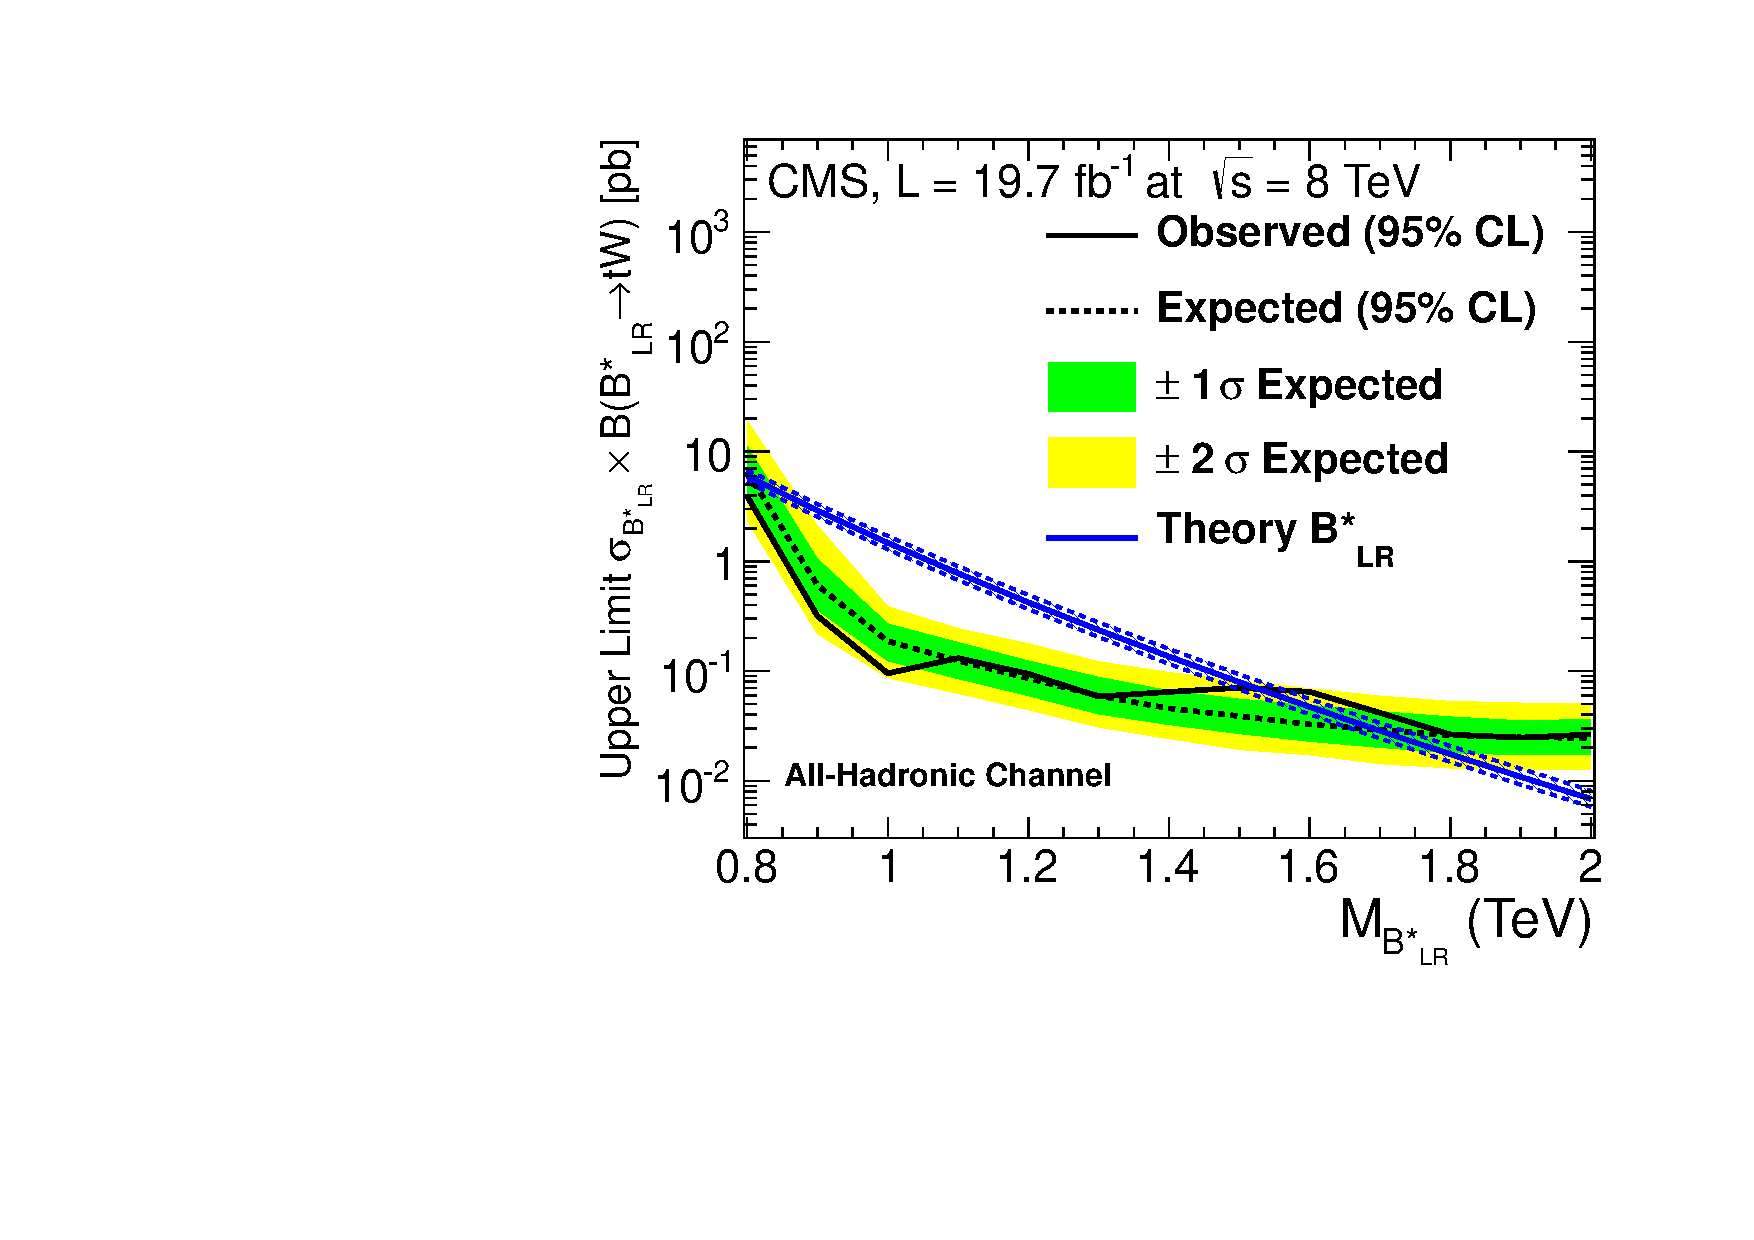
\includegraphics[width=0.45\textwidth]{AN-14-049/figs/limits_theta_had_vector_log.pdf}
\caption{The $\bs$ quark 95\% C.L. production cross-section limits.  The expected (dashed black) and observed (solid black) limits as well as $\bs$ quark 
theoretical cross-section (blue) are plotted for comparison.  
The uncertainty in the expected limit band is shown in green ($\pm$1$\sigma$) and yellow ($\pm$2$\sigma$).
These limits were extracted using the Theta limit setting framework.  Here, the signal hypotheses of a right-handed, left-handed, and vectorlike $\bs$ quark are 
shown on the top, middle, and bottom plots respectively. }
\label{figs:bsthetalimit}
\end{figure}


\begin{figure}[htcb]
\centering
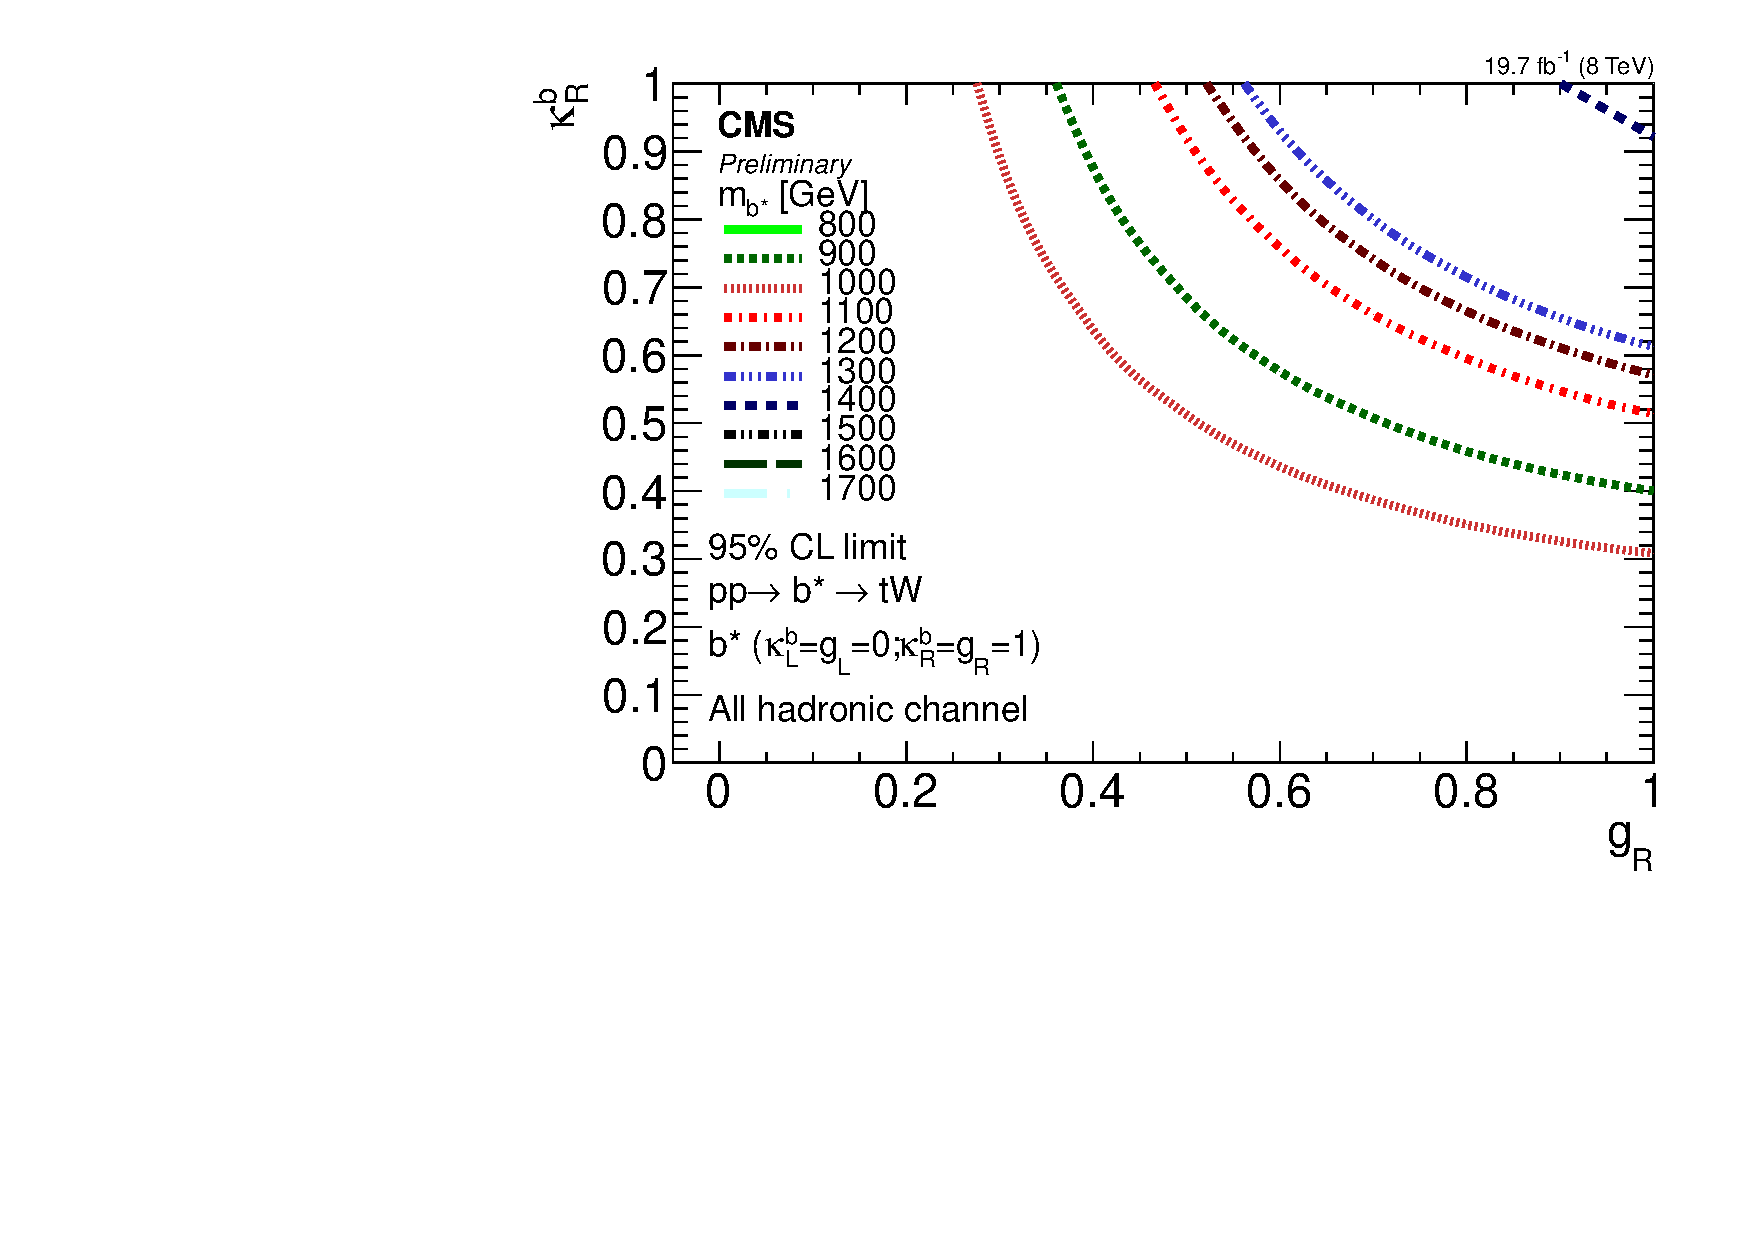
\includegraphics[width=0.5\textwidth]{AN-14-049/figs/bayesian_observed_hadronic_right_2Dlimit_plot.pdf}\\
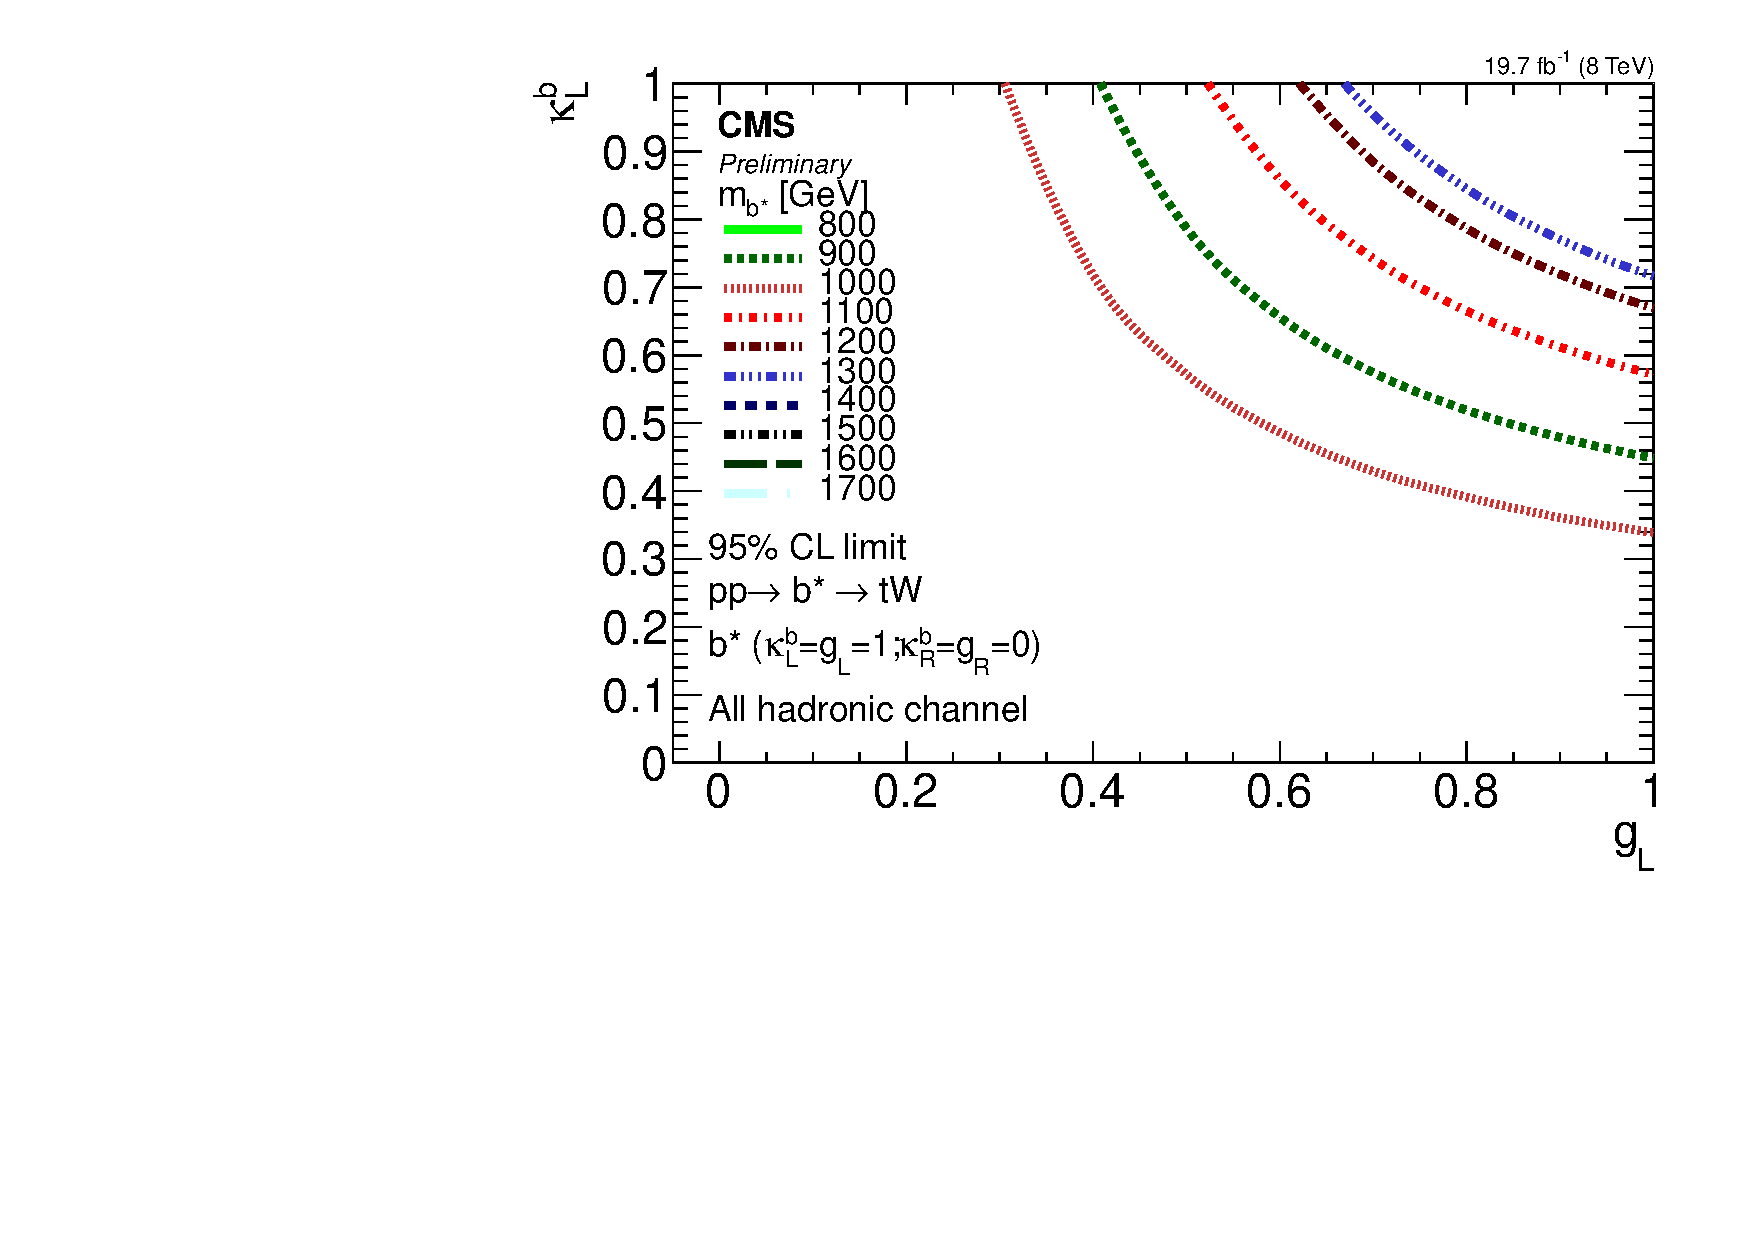
\includegraphics[width=0.5\textwidth]{AN-14-049/figs/bayesian_observed_hadronic_left_2Dlimit_plot.pdf}\\
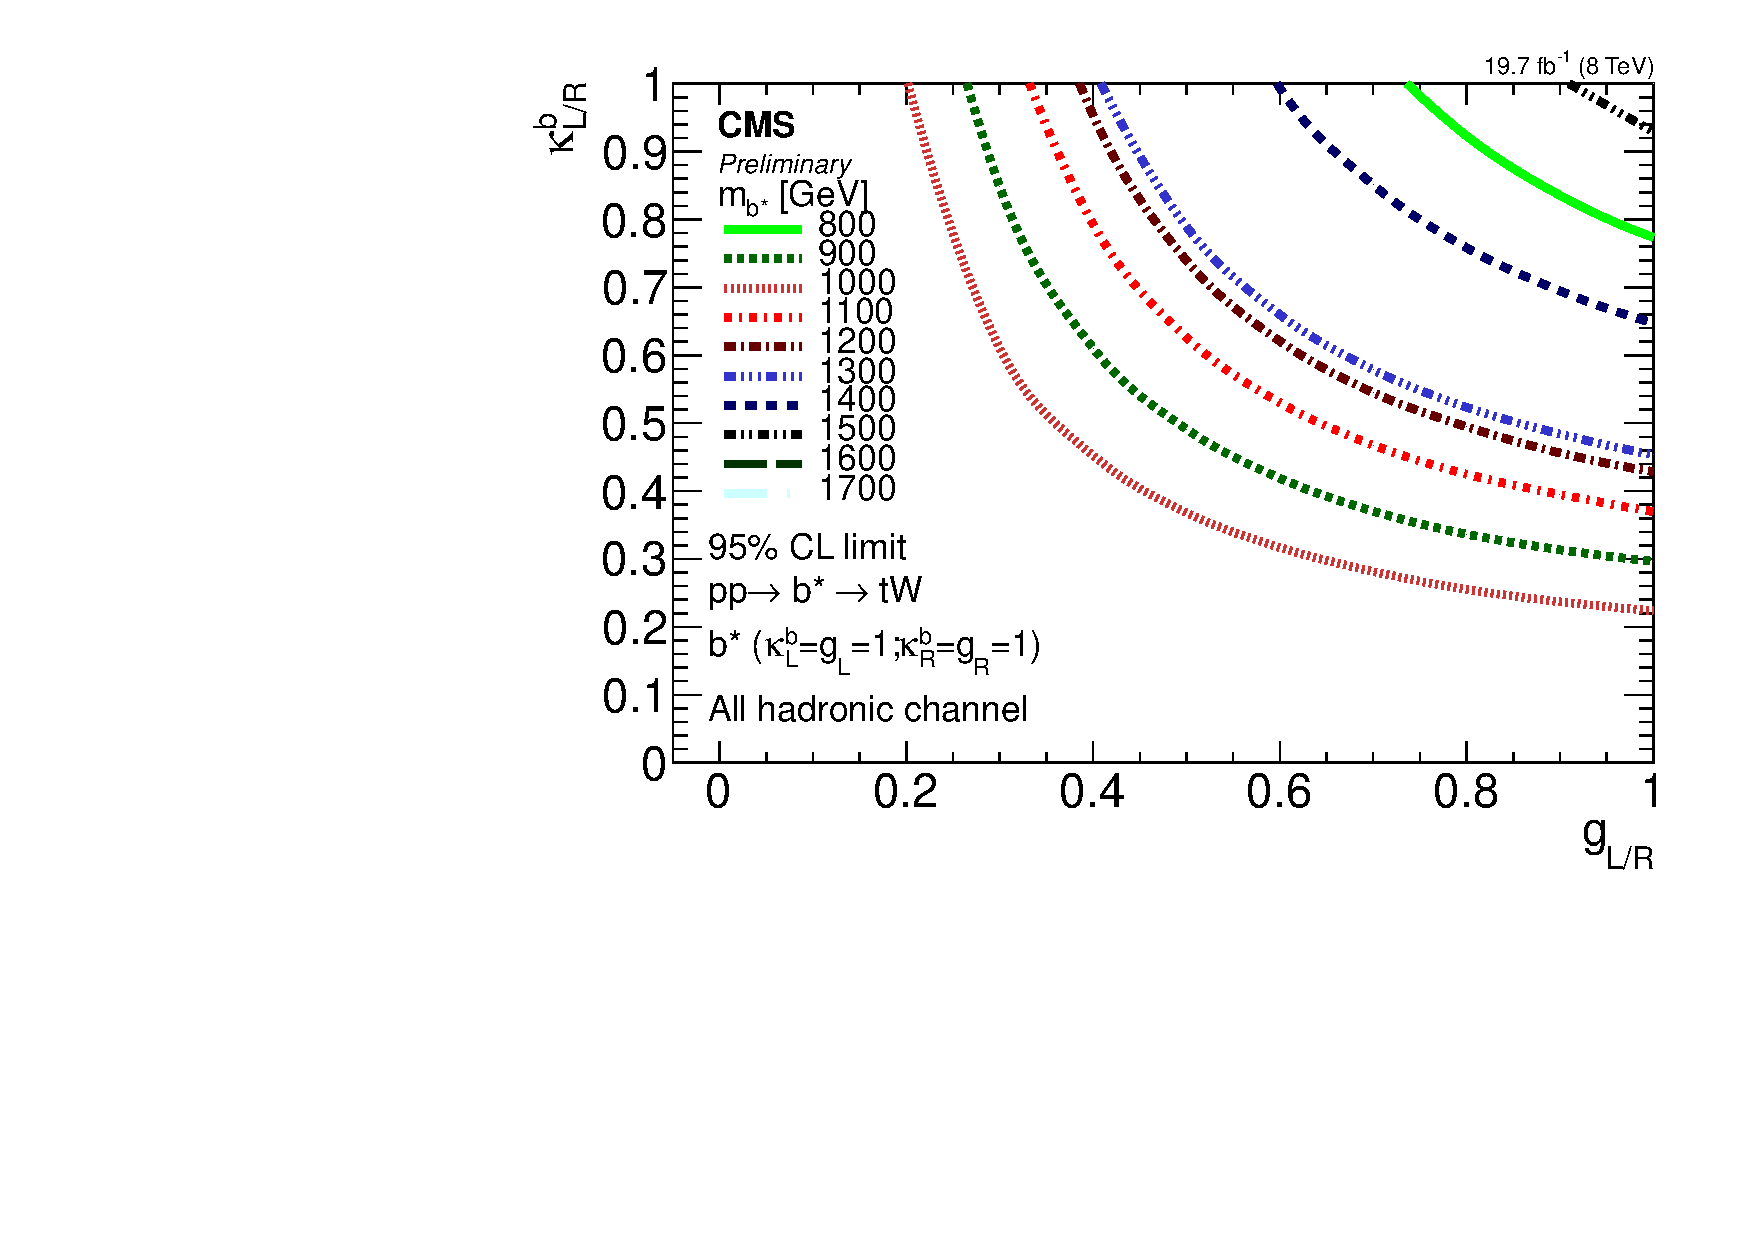
\includegraphics[width=0.5\textwidth]{AN-14-049/figs/bayesian_observed_hadronic_vector_2Dlimit_plot.pdf}\\
\caption{observed limit plot in the $\kappa$,$g$ plane.  The top, middle, and bottom plots show limits for right, left and vectorlike coupling hypotheses respectively.}
\label{figs:bsthetalimit2dobs}
\end{figure}


\begin{figure}[htcb]
\centering
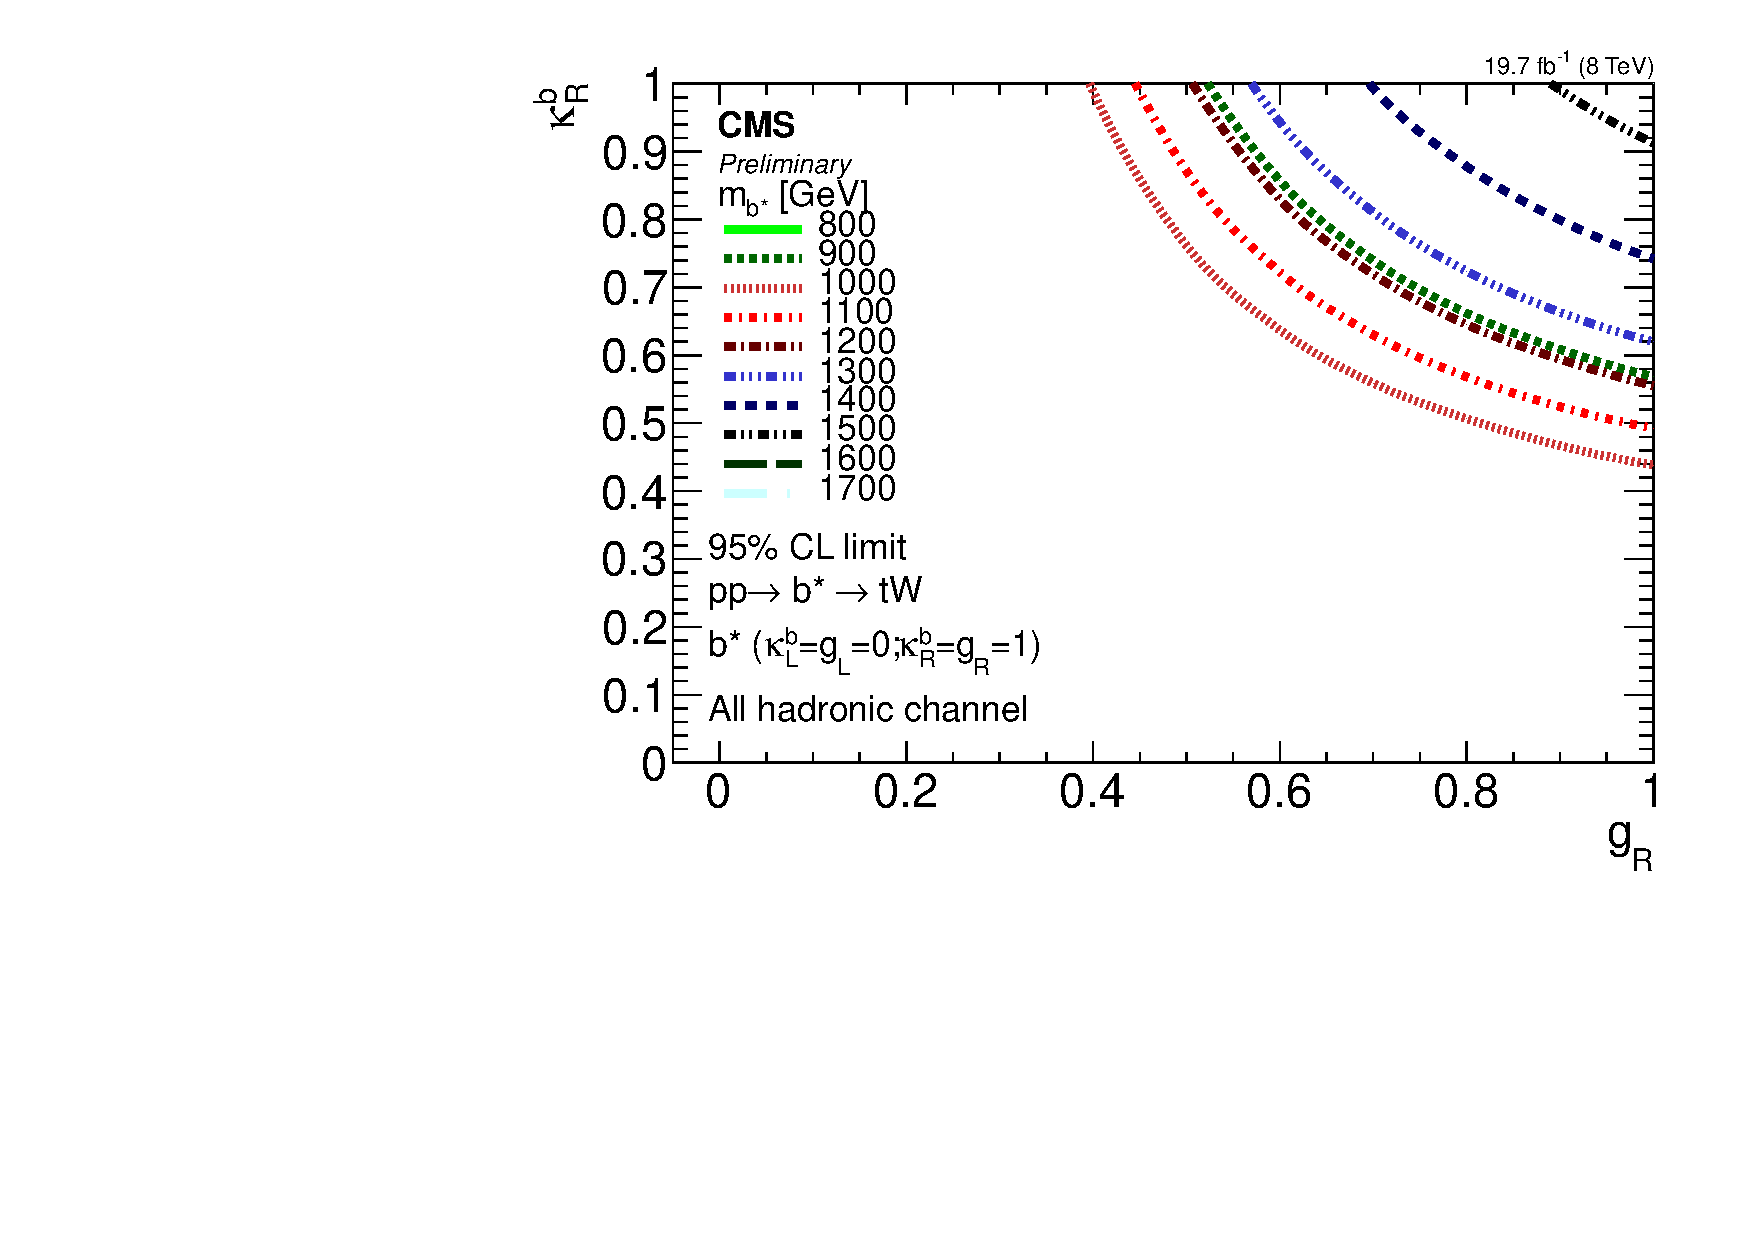
\includegraphics[width=0.5\textwidth]{AN-14-049/figs/bayesian_expected_hadronic_right_2Dlimit_plot.pdf}\\
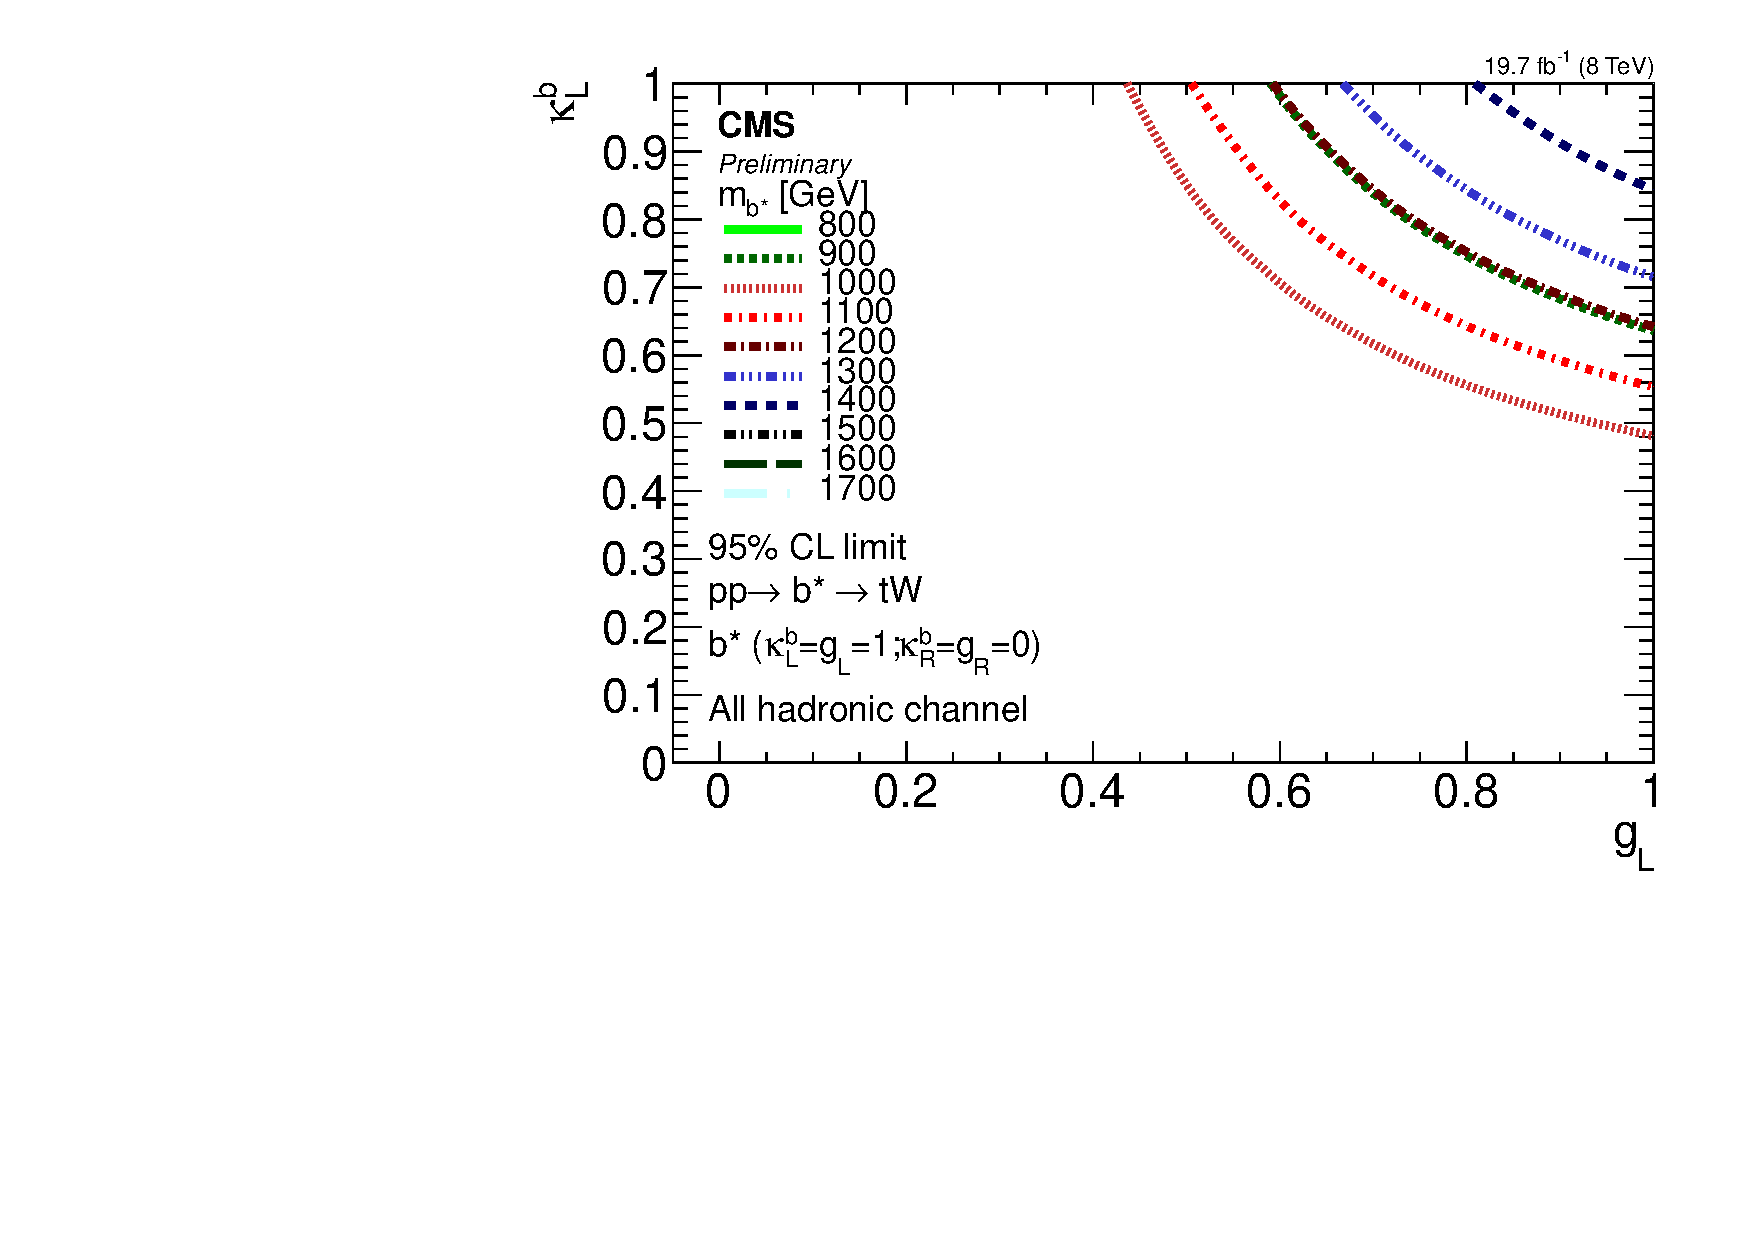
\includegraphics[width=0.5\textwidth]{AN-14-049/figs/bayesian_expected_hadronic_left_2Dlimit_plot.pdf}\\
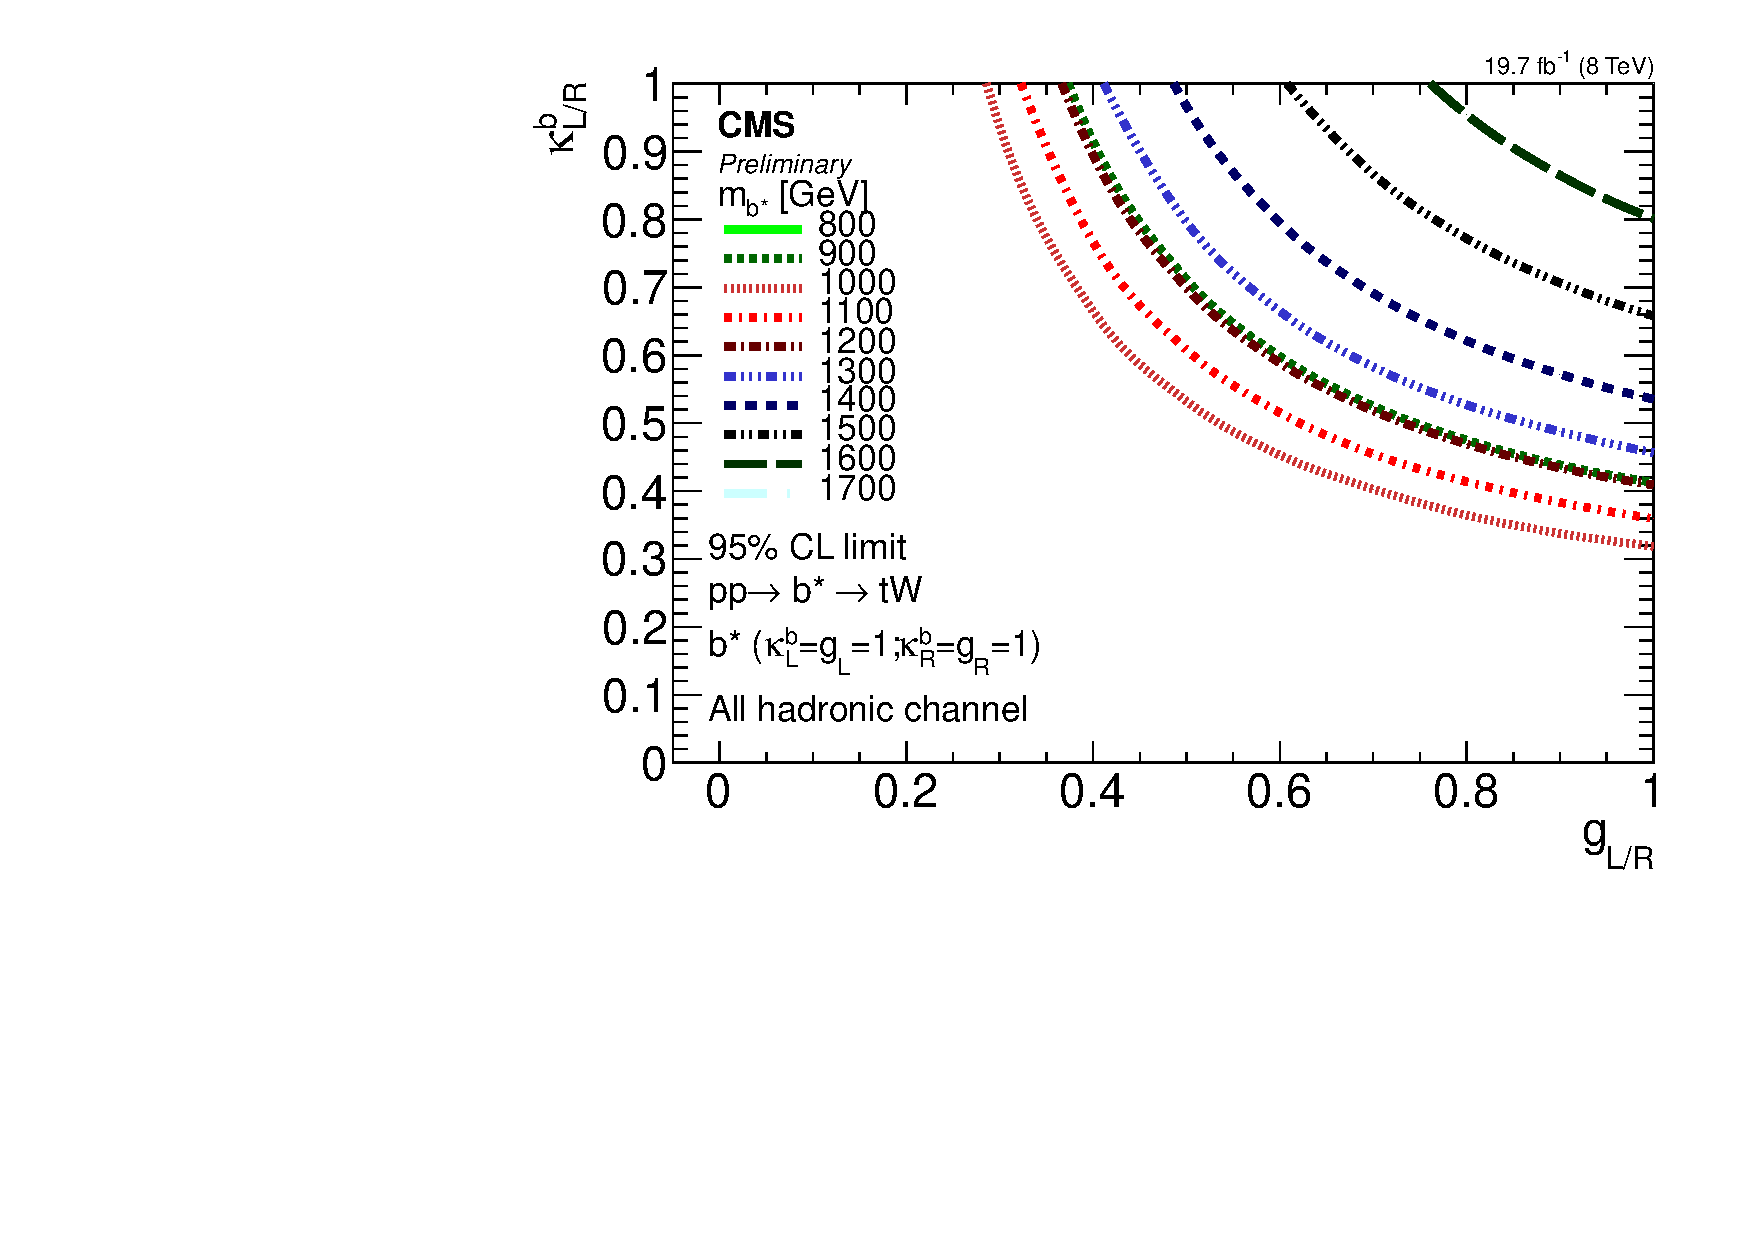
\includegraphics[width=0.5\textwidth]{AN-14-049/figs/bayesian_expected_hadronic_vector_2Dlimit_plot.pdf}\\
\caption{expected limit plot in the $\kappa$,$g$ plane.  The top, middle, and bottom plots show limits for right, left and vectorlike coupling hypotheses respectively.}
\label{figs:bsthetalimit2dexp}
\end{figure}

%\begin{sidewaystable}
%\begin{center}
%\bf{Nuisance Parameters}\\
%\scalebox{0.65}{
%\begin{tabular}{|c||c|c|c|c|c|c|c|c|c|c|c|}
%\hline
%\hline
%\end{tabular}
%}
%\end{center}
%\caption{Nuisance parameters after the fit.  This the nominal value found for the nuisance parameter after the fit in units of input sigma.}
%\label{table:bsnuisance}
%\end{sidewaystable}


\clearpage
